\documentclass[border=4pt]{standalone}
\usepackage{tikz}
\usepackage{pgfplots}
\pgfplotsset{compat=1.18}
\usetikzlibrary{shapes.geometric,arrows.meta,positioning,calc,fit,decorations.pathreplacing,backgrounds}
\definecolor{boxblue}{RGB}{225,238,252}
\definecolor{boxgreen}{RGB}{225,247,231}
\definecolor{boxorange}{RGB}{253,236,216}
\definecolor{boxgray}{RGB}{237,237,237}
\definecolor{boxred}{RGB}{253,226,226}
\begin{document}
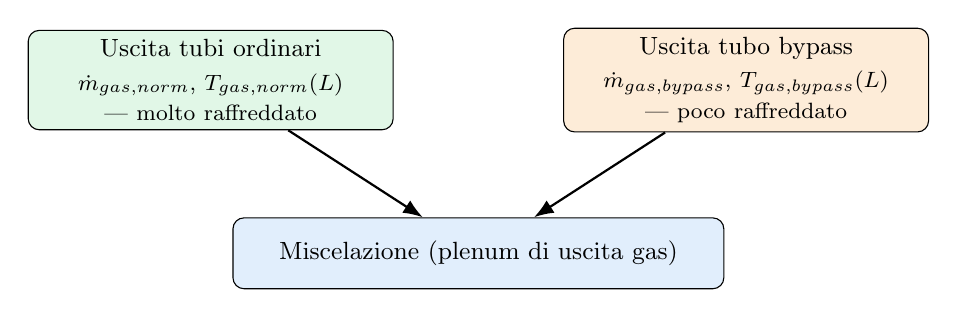
\begin{tikzpicture}[
  box/.style={draw, rectangle, rounded corners, minimum height=0.9cm, text width=4.4cm, align=center, font=\small},
  arr/.style={-{Latex[length=2.5mm]}, thick}
]
\node[box, fill=boxgreen] (t1) at (-3.4,1.4) {Uscita tubi ordinari\\[1pt]\footnotesize $\dot m_{gas,norm}$, $T_{gas,norm}(L)$ — molto raffreddato};
\node[box, fill=boxorange] (t2) at (3.4,1.4) {Uscita tubo bypass\\[1pt]\footnotesize $\dot m_{gas,bypass}$, $T_{gas,bypass}(L)$ — poco raffreddato};
\node[box, fill=boxblue, text width=6cm] (mix) at (0,-0.8) {Miscelazione (plenum di uscita gas)};

\draw[arr] (t1) -- (mix);
\draw[arr] (t2) -- (mix);
\end{tikzpicture}
\end{document}
